\documentclass[tikz, border = 0.01 cm]{standalone}
% Math font
\usepackage{amsthm}
\usepackage{amsmath}
\usepackage{amsfonts}
\usepackage{amssymb}
\usepackage{physics}

% TikZ and page libraries
\usepackage{xcolor}
\usepackage{tikz}
\usepackage{tkz-euclide}
\usepackage{pdfpages}

\usetikzlibrary{calc, patterns, angles, quotes, decorations.markings, decorations.pathreplacing, calligraphy}

\begin{document}

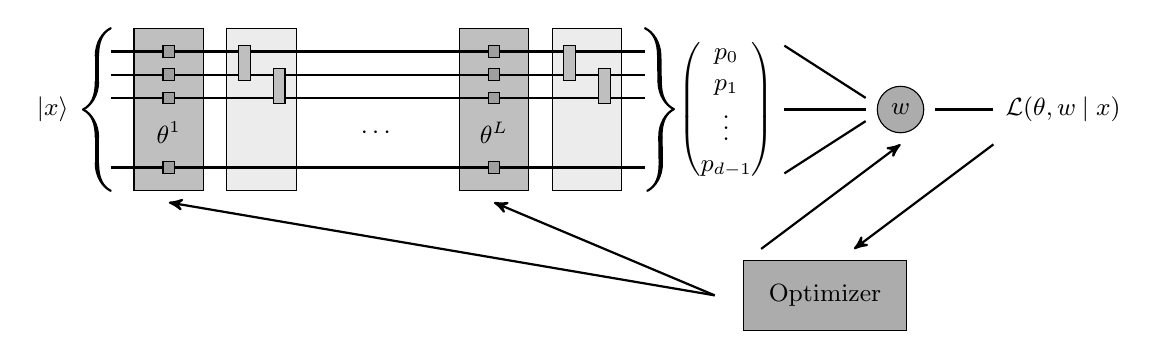
\begin{tikzpicture}[scale = 0.59]
    \filldraw[fill = gray!50] (+0.000, -1.750) rectangle (+1.500, +1.750);
    %
    \filldraw[fill = gray!15] (+2.000, -1.750) rectangle (+3.500, +1.750);
    
    \filldraw[fill = gray!50] (7.000 +0.000, -1.750) rectangle (7.000 + 1.500, +1.750);
    %
    \filldraw[fill = gray!15] (7.000 +2.000, -1.750) rectangle (7.000 + 3.500, +1.750);
    
    \draw[ultra thick, decorate, decoration = {calligraphic brace, amplitude = 10 pt}] (-0.500, -1.750) -- (-0.500, +1.750);
    
    % Lines
    \draw[thick] (-0.500, +1.250) -- (+11.000, +1.250);
    %
    \draw[thick] (-0.500, +0.750) -- (+11.000, +0.750);
    %
    \draw[thick] (-0.500, +0.250) -- (+11.000, +0.250);
    
    \draw[thick] (-0.500, -1.250) -- (+11.000, -1.250);
    
    \draw[ultra thick, decorate, decoration = {calligraphic brace, amplitude = 10 pt, mirror}] (+11.050, -1.750) -- (+11.000, +1.750);
    
    \node at (-1.750, +0.000) {\small{$| x \rangle$}};
        
    \node at (+12.750, +0.000) {\small{$\begin{pmatrix} p_{0} \\ p_{1} \\ \vdots \\ p_{d - 1} \end{pmatrix}$}};
    
    \node at (+0.750, -0.500) {\small{$\theta^{1}$}};
    %
    \node at (+7.750, -0.500) {\small{$\theta^{L}$}};
    
    \filldraw[fill = gray!75] (+0.625, +1.125) rectangle (+0.875, +1.375);
    %
    \filldraw[fill = gray!75] (+0.625, +1.125 - 0.500) rectangle (+0.875, +1.375 - 0.500);
    %
    \filldraw[fill = gray!75] (+0.625, +1.125 - 1.000) rectangle (+0.875, +1.375 -1.000);
    %
    \filldraw[fill = gray!75] (+0.625, +1.125 - 2.500) rectangle (+0.875, +1.375 -2.500);
    
    \filldraw[fill = gray!75] (7.000 + 0.625, +1.125) rectangle (7.000 + 0.875, +1.375);
    %
    \filldraw[fill = gray!75] (7.000 + 0.625, +1.125 - 0.500) rectangle (7.000 + 0.875, +1.375 - 0.500);
    %
    \filldraw[fill = gray!75] (7.000 + 0.625, +1.125 - 1.000) rectangle (7.000 + 0.875, +1.375 -1.000);
    %    
    \filldraw[fill = gray!75] (7.000 + 0.625, +1.125 - 2.500) rectangle (7.000 + 0.875, +1.375 -2.500);
    
    \filldraw[fill = gray!50] (+2.250, +1.125 - 0.500) rectangle (+2.500, +1.375);
    
    \filldraw[fill = gray!50] (+3.000, +1.125 - 1.000) rectangle (+3.250, +0.875);
    
    \filldraw[fill = gray!50] (+2.250 + 7.000, +1.125 - 0.500) rectangle (+2.500 +7.000, +1.375);
    
    \filldraw[fill = gray!50] (+3.000 + 7.000, +1.125 - 1.000) rectangle (+3.250 + 7.000, +0.875);
    
    \node at (+5.250, -0.500) {\small{$\cdots$}};
    
    \draw[thick] (+14.000, -1.375) -- (+15.750, -0.250);
    %
    \draw[thick] (+14.000, +0.000) -- (+15.750, +0.000);
    %
    \draw[thick] (+14.000, +1.375) -- (+15.750, +0.250);
    
    \draw[thick] (+17.250, +0.000) -- (+18.500, +0.000);
    
    \filldraw[fill = gray!65] (+16.500, +0.000) circle [radius = 0.5 cm];
    
    \node at (+16.500, +0.000) {\small{$w$}};
    
    \node at (+20.000, +0.000) {\small{$\mathcal{L}(\theta, w \: | \; x)$}};
    
    \filldraw[fill = gray!65] (+13.125, -4.750) rectangle (+16.625, -3.250);
    %
    \node at (+14.875, -4.000) {\small{Optimizer}};
    
    \draw[thick, -stealth'] (+12.500, -4.000) -- (+0.750, -2.000);
    %
    \draw[thick, -stealth'] (+12.500, -4.000) -- (+7.750, -2.000);
    %
    \draw[thick, -stealth'] (+13.500, -3.000) -- (+16.500, -0.750);
    %
    \draw[thick, stealth'-] (+13.500 + 2.000, -3.000) -- (+16.500 + 2.000, -0.750);
\end{tikzpicture}

\end{document}
